%%%%%%%%%%%%%%%%%%%%%%%%%%%%%%%%%%%%%%%%%%%%%%%%%%%%%%%%%%%%%%%%%%%%%%%%%%%%%%%%
%%%%%%%%%%%%%%%%%%%%%%%%%%%%%%%%%%%%%%%%%%%%%%%%%%%%%%%%%%%%%%%%%%%%%%%%%%%%%%%%
%%% Template for AIMS Rwanda Assignments         %%%              %%%
%%% Author:   AIMS Rwanda tutors                             %%%   ###        %%%
%%% Email: tutors2017-18@aims.ac.rw                               %%%   ###        %%%
%%% Copyright: This template was designed to be used for    %%% #######      %%%
%%% the assignments at AIMS Rwanda during the academic year %%%   ###        %%%
%%% 2017-2018.                                              %%%   #########  %%%
%%% You are free to alter any part of this document for     %%%   ###   ###  %%%
%%% yourself and for distribution.                          %%%   ###   ###  %%%
%%%                                                         %%%              %%%
%%%%%%%%%%%%%%%%%%%%%%%%%%%%%%%%%%%%%%%%%%%%%%%%%%%%%%%%%%%%%%%%%%%%%%%%%%%%%%%%
%%%%%%%%%%%%%%%%%%%%%%%%%%%%%%%%%%%%%%%%%%%%%%%%%%%%%%%%%%%%%%%%%%%%%%%%%%%%%%%%


%%%%%% Ensure that you do not write the questions before each of the solutions because it is not necessary. %%%%%% 

\documentclass[12pt,a4paper]{article}

%%%%%%%%%%%%%%%%%%%%%%%%% packages %%%%%%%%%%%%%%%%%%%%%%%%
\usepackage{amsmath}
\usepackage{amssymb}
\usepackage{amsthm}
\usepackage{amsfonts}
\usepackage{graphicx}
\usepackage[all]{xy}
\usepackage{tikz}
\usepackage{verbatim}
\usepackage{float}
\usepackage[left=2cm,right=2cm,top=3cm,bottom=2.5cm]{geometry}
\usepackage{hyperref}
\usepackage{caption}
\usepackage{subcaption}
\usepackage{psfrag}

%%%%%%%%%%%%%%%%%%%%% students data %%%%%%%%%%%%%%%%%%%%%%%%
\newcommand{\student}{Yuusf Brima}
\newcommand{\course}{Partial Differential Equations}
\newcommand{\assignment}{1}

%%%%%%%%%%%%%%%%%%% using theorem style %%%%%%%%%%%%%%%%%%%%
\newtheorem{thm}{Theorem}
\newtheorem{lem}[thm]{Lemma}
\newtheorem{defn}[thm]{Definition}
\newtheorem{exa}[thm]{Example}
\newtheorem{rem}[thm]{Remark}
\newtheorem{coro}[thm]{Corollary}
\newtheorem{quest}{Question}[section]

%%%%%%%%%%%%%%  Shortcut for usual set of numbers  %%%%%%%%%%%

\newcommand{\N}{\mathbb{N}}
\newcommand{\Z}{\mathbb{Z}}
\newcommand{\Q}{\mathbb{Q}}
\newcommand{\R}{\mathbb{R}}
\newcommand{\C}{\mathbb{C}}

%%%%%%%%%%%%%%%%%%%%%%%%%%%%%%%%%%%%%%%%%%%%%%%%%%%%%%%555
\begin{document}

%%%%%%%%%%%%%%%%%%%%%%% title page %%%%%%%%%%%%%%%%%%%%%%%%%%
\thispagestyle{empty}
%\begin{figure}
%    \centering
%    \includegraphics[width=\textwidth]{aims_rwanda.jpg}
%\end{figure}
\begin{center}
\textbf{AFRICAN INSTITUTE FOR MATHEMATICAL SCIENCES \\[0.5cm]
(AIMS RWANDA, KIGALI)}
\vspace{1.0cm}
\end{center}

%%%%%%%%%%%%%%%%%%%%% assignment information %%%%%%%%%%%%%%%%
\noindent
\rule{17cm}{0.2cm}\\[0.3cm]
Name: \student \hfill Assignment Number: \assignment\\[0.1cm]
Course: \course \hfill Date: \today\\
\rule{17cm}{0.05cm}
\vspace{1.0cm}
\section{The Green’s function for the IVP}
\begin{equation}
	y^{\prime \prime} +p(x)y^\prime +q(x)y=r(x) \quad,   \text{with } y(0)=0 \text{ and }   y^\prime(0)=0
	\label{eq:1}
\end{equation}
is given by
\begin{equation}
   G(x,s) = \frac{y_1(s)y_2(x) - y_1(x)y_2(s)}{W[y_1,y_2](s)}
   \label{eq:2}
\end{equation}
where $ y_1$ and $ y_2$ are independent solutions of the homogeneous equation
\begin{equation}
	y^{\prime \prime} + p(x)y^\prime + q(x)y = 0
	\label{eq:3}
\end{equation}
\begin{enumerate}
	\item[(a)] Functions
		\begin{align*}
			\tilde{y}_1(x) = ay_1(x) + by_2(x)\\
			\tilde{y}_2(x) = cy_1(x) + dy_2(x)
		\end{align*}
	 are also solutions of \eqref{eq:3}.  Give a condition on $a, b, c$ and $d$ which make $\tilde{y}_1(x)$ and $\tilde{y}_2x)$ independent solutions.
Differentiating the equations for  $\tilde{y}_1(x)$ and $\tilde{y}_2x)$ we obtain
		\begin{align*}
			\tilde{y}_1(x) = ay_1^\prime(x) + by_2^\prime(x)\\
			\tilde{y}_2(x) = cy_1^\prime(x) + dy_2^\prime(x)
		\end{align*}
	Substituting this into $ W[\tilde{y}_1,\tilde{y}_2]$ gives after a small amount of algebra
	\begin{align*}
		W[\tilde{y}_1^,\tilde{y}_2^] = (ad - bc) (y_1y_2^\prime - y_2y_1^\prime) = (ad - bc)W[y_1,y_2]
	\end{align*}
	Since $y_1$ and $y_2$ are independent solutions we know that $W [y1 , y2 ](x) \neq 0.$ Hence 
	\begin{align*}
		W[\tilde{y}_1,\tilde{y}_2]  \neq 0 \iff  ad - bc \neq  0
	\end{align*}
	
	Note that this is simply the condition that the linear transformation relating $	\tilde{y}_1^\prime, 	\tilde{y}_2^\prime$ to $y_1, y_2$
has non-zero determinant and is therefore invertible.
\item[(b)] Using the above equations we calculate that
\begin{align*}
		\tilde{y}_1(s)\tilde{y}_2(x) - \tilde{y}_1(x)\tilde{y}_2(s)  = (ad -bc){y_2(s) y_2(x) - y_1(x)y_2(s)}
	\end{align*}
	We already know that
	\begin{align*}
				W[\tilde{y}_1,\tilde{y}_2](s) = (ad - bc)W [y_1, y_2](s)
		\end{align*}
	
	So that using formula \eqref{eq:2} but with $\tilde{y}_1$ and $$\tilde{y}_2$$ gives:
	
	\begin{align*}
	    \frac{\tilde{y}_1(s)\tilde{y}_2(x) - \tilde{y}_1(x)\tilde{y}_2(s)}{W[\tilde{y}_1,\tilde{y}_2]}(s)  &= \frac{(ad - bc){y_1(s)y_2(x) - y_1(x)y_2(s)}}{(ad - bc)W[y_1,y_2](s)}\\
	    &= \frac{y_1(s)y_2(x) - y_1(x)y_2(s)}{W[y_1,y_2](s)} \quad \text{Since} (ad - bc) \neq 0\\
	    &= G(x,s)
	\end{align*}
So that the Green’s function constructed from $\tilde{y}_1$ and $\tilde{y}_2$ is identical to that constructed
from $y_1$ and $y_2$.
\item[(c)] To Green’s function for the IVP
    \begin{align*}
        y^{\prime \prime} - 4y^\prime + 4y = r(x) \quad \text{ with } y(0)=0 \text{ and } y\prime(0)=0
    \end{align*}
    and use this to obtain the solution to the above problem when $r(x) = xe^{2x}$.
The homogeneous equation is
    \begin{align*}
        y^{\prime \prime} - 4y^\prime + 4y = 0
    \end{align*}
with characteristic equation
    \begin{align*}
        m^2 - 4m + 4 = 0
    \end{align*}

This is just $(m - 2)^2 = 0$ so that the solution is $m = 2$ (twice). We may therefore take $y_1(x) = e^{2x}$ and $y2(x) = xe^{2x}$ as independent solutions of the homogeneous equation. The Wronskian is given by
\begin{align*}
    W[y_1,y_2](x) = \begin{vmatrix}
                    e^{2x} & xe^{2x} \\ 
                    2e^{2x} & e^{2x} + 2xe^{2x}
                    \end{vmatrix}
\end{align*}
Hence substituting into equation \eqref{eq:2} gives:
\begin{align*}
    G(x, s) = \frac{e^{2s}xe^{2x} -  e^{2x}se^{2s}}{e^{4s}} = xe^{2x}e^{-2s} - e^{2x}se^{-2s}
\end{align*}
Note (although we will not use this fact below) that we can write the above as $G(x, s) = (x - s)e^{2(x-s)}$ so that $G(x, s)$ can be written as a function of $(x - s)$.
To solve the equation $y^{\prime \prime} - 4y^\prime + 4y = xe^{2x}$ with $y(0)=0$ and $y\prime (0)=0 $ we use the Green’s function calculated above and $r(x) = xe^{2x}$
\begin{align*}
    y(x) &= \int_{s=0}^{s=x} G(x,s)r(s) ds\\
        &= \int_{s=0}^{s=x} (xe^{2x}e^{-2s} - e^{2x}se^{-2s})se^{2s} ds\\
        &= xe^{2x} \int_{s=0}^{s=x} sds  - e^{2x} \int_{s=0}^{s=x} s^2 ds\\
        &= xe^{2x}(\frac{x^2}{2}) - e^{2x}(\frac{x^3}{3})\\
        &= (\frac{x^3}{6})e^{2x}
\end{align*}
So that the required solution is $y(x) =  (\frac{x^3}{6})e^{2x}$.
\section*{Exercise 2}
\begin{enumerate}
    \item[(a)]
        Given a boundary value problem,
\begin{align}
y{''}= \lambda y,  \hspace{0.5cm} y(0) =0, \hspace{0.5cm}  y'(1) = 0, \hspace{0.5cm} x\in [0,1].
\label{eq}
\end{align}
In this subsection, required is to show that
\begin{align}
\int_{0}^{1} (y_{m}(x)y''_{n}(x)-y_{n}(x)y''_{m}(x))dx = 0
\label{aq}
\end{align}
We must prove equation \ref{aq} without calculating $y_{n}(x)$. Using integration by parts, and letting  $u_{1}(x) = y_{m}(x)$ , $u_{2}(x) = y_{n}(x)$ , $v'_{1} = y''_{n}(x)$ and $ v'_{2} = y''_{m}(x)$.\\
This therefore means that, $u'_{1}(x) = y'_{m}(x)$ , $u'_{2}(x) = y'_{n}(x)$ , $v_{1} = y'_{n}(x)$ and $ v_{2} = y'_{m}(x)$.
So, using the fact that $\int uv'dx = uv - \int vu'dx$, equation \ref{aq} becomes;
\begin{align}
[y_{m}(x)y'_{n}(x) - y_{n}(x)y'_{m}(x)]_{0}^{1} + \int_{0}^{1}(y'_n(x)y'_{m}(x) - y'_{m}(x)y'_{n}(x))dx
\label{at}
\end{align}
The term integrated over $[0,1]$ vanishes because it's equal to zero. This leaves equation \ref{at} as,
\begin{align*}
\bigg[y_{m}(x)y'_{n}(x) - y_{n}(x)y'_{m}(x)\bigg]_{0}^{1}
\end{align*}
Evaluating this gives, $[y_{m}(1)y'_{n}(1) - y_{n}(1)y'_{m}(1)] - [y_{m}(0)y'_{n}(0) - y_{n}(0)y'_{m}(0)]$. Using boundary conditions stated in equation \ref{eq} implies that \ref{aq} is true.\\\\
Therefore, $\int_{0}^{1} (y_{m}(x)y''_{n}(x)-y_{n}(x)y''_{m}(x))dx = 0$
\subsection*{Hence part}
Using the fact that $y''_{n}=\lambda _{n} y_{n}$ and $y''_{m}=\lambda _{m} y_{m}$. Equation \ref{aq} then becomes.
\begin{align*}
\int_{0}^{1} (\lambda_{n}y_{m}(x)y_{n}(x) - \lambda_{m}y_{m}(x)y_{n}(x))dx= 0
\end{align*}
This can be written as, $(\lambda_{n} - \lambda_{m})\int_{0}^{1}y_{m}(x)y_{n}(x) dx= 0 $.
For n$\ne$ m, $\implies$ $\int_{0}^{1}y_{m}(x)y_{n}(x) dx= 0 $

\item[(b)] 
In this subsection, required is to find the eigenvalues and eigenfunctions for the BVP given in equation \ref{eq}. Since $\lambda \in \R $ we shall proceed by looking at the possible cases. That is, when $\lambda =0, \lambda > 0$ and $\lambda < 0$.
\subsection*{Case (i)}
When $\lambda = 0 $; the ODE in equation \ref{eq} then becomes $y'' = 0$ with a solution given $ y(x)= Ax+B$ Where $A$ and $B$ are constants. Then, $y'(x)= A$. Applying BV conditions, $y(0)=0 \implies B=0$ and $y'(1)=0 \implies A=0$. This implies that for $\lambda = 0$ the solution is trivial $\forall$ x.
\subsection*{Case (ii)}
When $\lambda > 0$; if we define $\lambda := \mu ^2 $, then the general solution of the ODE in \ref{eq} becomes $$y(x) = Ae^{\mu x} + Be^{-\mu x},$$
Then $$ y'(x) = \mu (Ae^{\mu x} -  Be^{-\mu x}),$$
Applying BV conditions, $y(0) =0 \implies A+B = 0 \iff A= -B$ and for $y'(1)=0$ implies $ \mu (Ae^{\mu } -  Be^{-\mu }) = 0$
Since $A= -B$, then $\mu A(e^{\mu } - e^{-\mu }) = 0$. Because $\mu >0$, this means that $A = B = 0$ since $e^{\mu } - e^{-\mu } \ne 0 $ . There for the solution is trivial $\forall$ x.
\subsection*{Case (iii)}
When $\lambda < 0$; we define $\lambda := -\mu ^2$ The ODE in equation \ref{eq} then has a solution of the form $y(x) = A\cos(\mu x) + B\sin(\mu x)$. Applying boundary conditions; For $y(0) = 0$ $\implies$ $A=0$. This then means that our solution is, $y(x) = B\sin(\mu x)$ and so $y'(x) = B\mu \cos(\mu x)$; For $y'(1) = 0$, this means that $B\mu \cos (\mu ) = 0$.
A trivial solution is obtained when $B=0$. \\
When $B\ne 0$, a non-trivial solution is obtained. This is true only if $$\cos(\mu) = 0 \iff \mu = \frac{\pi}{2}, \frac{3\pi}{2},\frac{\pi}{2}+ 2\pi, \cdot \cdot$$
This means that for the solution to be non-trivial, $\mu_k = \frac{\pi}{2} + k\pi \hspace{0.5cm}; k\in \Z$.\\
For \textbf{eigenvalues}, we recall that $\lambda = -\mu^2 $ $\implies \lambda_n = -\bigg(\frac{(2n+1)\pi}{2}\bigg)^2$ \hspace{0.5cm} ; n$\in\N$\\\\
Given the non-trivial solutions, $y(x)= B\sin(\mu x)$, the \textbf{eigenfunctions} are given by; $$ y_{n}(x) = B\sin\bigg(\frac{(2n+1)\pi}{2}x\bigg) \hspace{0.5cm} ;n \in \N$$
The set of eigenvalues used to deduce the eigenfunctions if picked from $\N$ to attain a set of distinct eigenvalues with a minimum eigenvalue as asserted by Sturm-Liouville theory.\\\\
For the orthogonality condition, we recall that  $\int_{0}^{1}y_{m}(x)y_{n}(x) dx= 0 $. Substituting for $y_{m}(x)$ and $y_{n}(x)$, the eigenfunctions designed at the $m^{th}$ and $n^{th}$ eigenvalues respectively with $B=1$ gives,
$$\int_{0}^{1}sin\bigg(\frac{(2n+1)\pi}{2}x\bigg)\sin\bigg(\frac{(2m+1)\pi}{2}x\bigg)dx= 0$$

\item [(c).]We are required to calculate the Green's function for the IVP.
\begin{align}
y''-4y'+4y=r(x) \,\,\,\, with\,\,\,\,\,\ y(0)=0, \,\,\,\, and \,\,\,\,y'(0)=0
\label{yusu}
\end{align}

and hence to use it to obtain the solution to the above problem when $r(x) = xe^{2x}$.\\\\

Firstly we need to find the Solution for  homogeneous part $$y''-4y'+4y=0$$

Setting
\begin{align*}
y=e^{rx}\Longrightarrow y'=re^{rx}\Longrightarrow y''=r^2e^{rx}
\end{align*}

Thus the auxiliary x-tics equation for the problem is
\begin{align}
r^2 -4r+4=0 \Longleftrightarrow (r-2)(r-2)=0\Longrightarrow r=2
\end{align}

The problem has repeated root $(r=2)$. and therefore the solutions to the problem are $$y_1(x)=e^{2x} \,\,\,\,and\,\,\,\, y_2(x)=xe^{2x}$$.

$y_1$ and $y_2$ are the independent homogeneous equation's solution and from this two solutions we can obtain the Wroskian after getting the derivatives of $y_1$ and $y_2$.


\begin{align*}
y_1(x)=e^{2x}\Longrightarrow y'_1(x)=2e^{2x}
\end{align*}

Also

\begin{align*}
y_2(x)=xe^{2x}\Longrightarrow y'_2(x)=e^{2x}+2xe^{2x}
\end{align*}

Therefore;
\begin{align}
\begin{aligned}
W[y_1,y_2](x)&=y_1y'_2-y'_1y_2\\
&=e^{2x}(e^{2x}+2xe^{2x}) -2e^{2x}xe^{2x}\\
&=e^{4x}+2xe^{4x}-2xe^{4x}\\
&=e^{4x}
\end{aligned}
\end{align}

Therefore to calculate the Green's function, we refer from equation \ref{key}, which results to;
\begin{align*}
G(x,s) &= \frac{e^{2s}xe^{2x}-e^{2x}se^{2s}}{e^{4s}}\\\\
&=xe^{2x}e^{-2s}-se^{2x}e^{-2s}\\\\
G(x,s)&=(x-s)e^{2x}e^{-2s}
\end{align*}

Therefore, the Green's function  for the IVP is $$G(x,s)=(x-s)e^{2(x-s)}$$

$\bullet$ We also supposed to find the solution of \ref{yusu} when $r(x)=xe^{2x}$ using the obtained Green function;
From
\begin{align}
\begin{aligned}
y(x)&=\int_{s=0}^{x}G(x,s)r(s)ds\\\\
&=\int_{s=0}^{x}(x-s)e^{2x}e^{-2s}se^{2s}ds\\\\
&=\int_{s=0}^{x}(xe^{2x}-se^{2x})sds\\\\
&=\int_{s=0}^{x}xe^{2x}sds-\int_{s=0}^{x}s^2e^{2x}ds\\\\
&=xe^{2x}\int_{s=0}^{x}sds-e^{2x}\int_{s=0}^{x}s^2ds\\\\
&=xe^{2x}\bigg[\frac{s^2}{2}\bigg]_{0}^{x}-e^{2x}\bigg[\frac{s^3}{3}\bigg]_{0}^{x}\\\\
&=xe^{2x}\frac{x^2}{2}-e^{2x}\frac{x^3}{3}\\\\
&=\frac{x^3}{2}e^{2x}-\frac{x^3}{3}e^{2x}=\frac{x^3}{6}e^{2x} \\
\end{aligned}
\end{align}

$\therefore$ The solution to the equation \eqref{yusu} is $$y(x)= \frac{x^3}{6}e^{2x} $$
\end{enumerate}
\end{enumerate}

\section*{Exercise 3}
\begin{enumerate}
    \item[(a)]  Graphical representation
            \begin{figure}[!h]
                \centering
                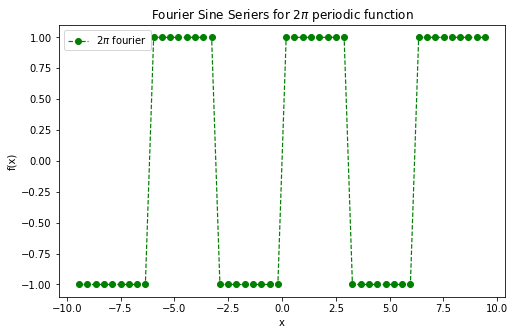
\includegraphics[width=350pt,height=250pt]{fourier.png}
                \caption{Graph of the function $f(x)$ for $-3\pi \leq x \leq 3 \pi$}
                \label{fig:my_label}
            \end{figure}
    \item[(b)]
        Given is a $2\pi$-periodic function, $f(x)$  defined on the interval $-\pi \leq x \leq \pi$.\\Required is to explain why this function $f(x)$ has a Fourier Sine series. \\
     By definition, the general Fourier Series is given by;

\begin{align}\label{eqt1}
f(x) &= \frac{a_0}{2} + \sum_{n=1}^{\infty} \{ a_n \cos (nx) + b_n \sin (nx)\} \hspace*{1cm} \\
\nonumber
\end{align}

In order to show tst this is true, we compute the value of the constant, $a_n$ and show that $a_n=0$ $\forall n\in \N$\\By defiinition, $a_n$ is given by;
\begin{align}\label{eqtn2}
a_n &= \frac{1}{\pi} \int_{-\pi}^{\pi} f(x) \cos (nx) dx\\
\nonumber
\end{align}
For our piece wise function, we have
\begin{align*}
a_n&= \frac{1}{\pi} \left[ \int_{-\pi}^{0} (-1) \cos (nx) dx + \int_{0}^{\pi} (1) \cos (nx) dx\right]\\
\nonumber
&= \frac{1}{\pi} \left[-\frac{\sin (0)}{n} + \frac{\sin n(-\pi)}{n} +\frac{\sin (n\pi)}{n}-\frac{\sin (0)}{n}\right]\\
\nonumber
&= 0\\
\nonumber
\end{align*}
Also, one can see this minus computing the integral. for an odd function, $f(-x) = -f(x)$. but $\cos(x)$ is an \textbf{even function} ($\cos (-nx) = \cos(nx)$), so the integral of $f(x)\cos(nx)$ is an \textbf{odd function}. This means that the integral over our piece wise intervals (-$\pi\le x \le 0$ and $0\le x \le \pi$) will cancel out to leave $a_n$ as zero.\\
This therefore proves the fact that $f(x)$ has a Fourier Sine series.r $\forall n\in \N$

\item[(c)]
    In this section, required is to calculate the Fourier series for $f(x)$. Since its known to be a Fourier sine series, it suffices to find the value of the constant $b_n$. By definition, it's known that,
\begin{align*}
b_n &= \frac{1}{\pi} \int_{-\pi}^{\pi} f(x) \sin (nx) dx\\
\nonumber
\implies b_n&= \frac{1}{\pi} \left[ \int_{-\pi}^{0} (-1) \sin (nx) dx + \int_{0}^{\pi} (1) \sin (nx) dx\right]\\
\nonumber
&= \frac{1}{\pi} \left[\frac{\cos (nx)}{n}\right]_{-\pi}^{0} + \frac{1}{\pi} \left[-\frac{\cos (nx)}{n}\right]_{0}^{\pi}\\
&= \frac{1}{\pi n} \left[ 1-(-1)^{n}-(-1)^{n}+1\right]\\
\nonumber
&= \frac{2}{\pi n} \left[ 1-(-1)^{n}\right]\\
\nonumber
\end{align*}
The above result is true since $\cos(0)=1$ and $\cos(-nx)=\cos(nx)= (-1)^n$.\\
With $b_n$ known, equation \eqref{eqt1} then becomes;

\begin{align*}
f(x) &= \frac{2}{\pi} \sum_{n=1}^{\infty} \bigg[\frac{1-(-1)^{n}}{n} \sin (nx)\bigg] \\
\nonumber
\end{align*}
Which is the Fourier sine series for the piece wise function in question.
\end{enumerate}

\end{document}